%=========================================================================
% (c) 2011, 2012 Josef Lusticky

\section{Network communication}
Thanks to uIP, described in section~\ref{sec:contiki-uip},
the network communication is not a matter for Contiki OS.

intended to be used between different processes

AVR Raven features IEEE~802.15.4 (Low-Rate Wireless Personal Area Networks) link layer support.
On top of this layer, an adaptation layer called 6LoWPAN (IPv6 over Low power Wireless Personal Area Networks)
is used to communicate over IPv6 by Contiki.

Figure~\ref{fig:design-6lowpan} shows a complete hierarchy of network layers
concerned with NTP communication.
\begin{figure}
  \centering
  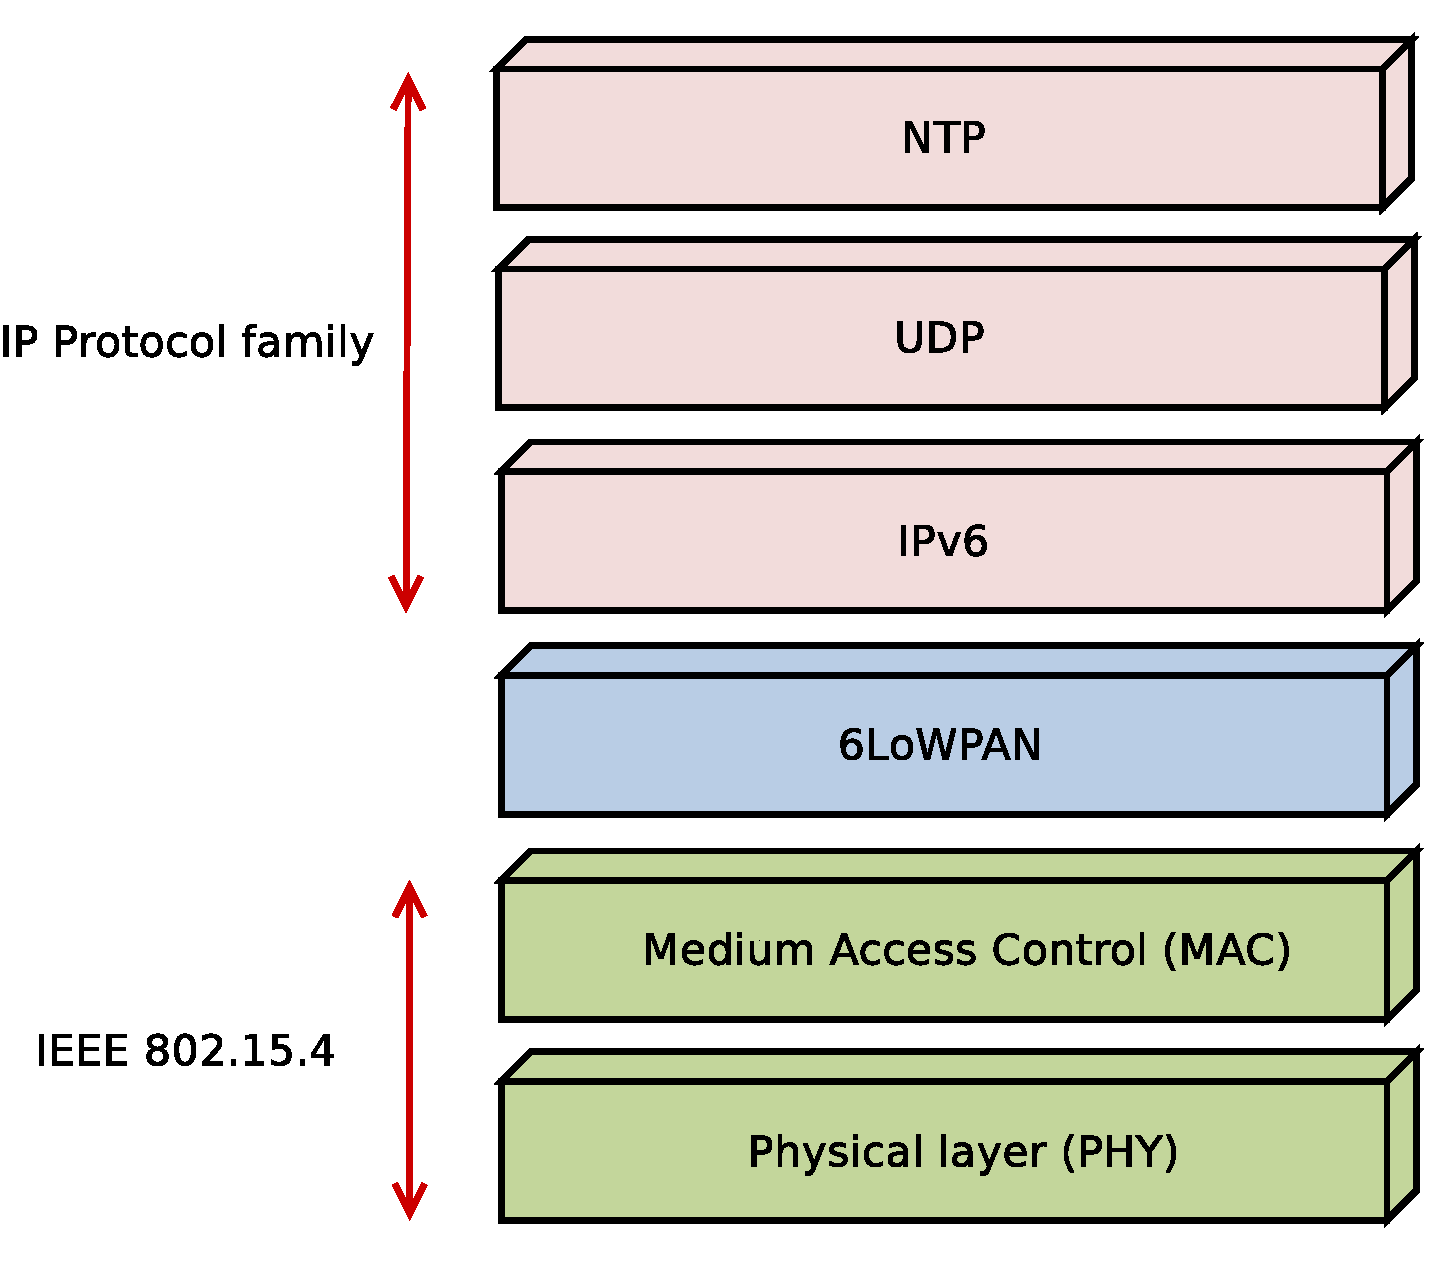
\includegraphics[width=9cm,keepaspectratio]{fig/6lowpan.pdf}
  \caption{Communication stack with 6lowpan layer}
  \label{fig:design-6lowpan}
  \bigskip
\end{figure}


